\documentclass[a4paper]{article}
\usepackage{fontspec}
\usepackage[russian]{babel}
\usepackage{listings}
\usepackage[a4paper]{geometry}
\usepackage{indentfirst}
\usepackage{graphicx}
\usepackage{caption}

\setmainfont{CMU Serif}
\setsansfont{CMU Sans Serif}

\begin{document}

\title{Лабораторная работа 1 по курсу <<Нелинейная динамика и её приложения>>. \\Отчёт.}
\author{Владислав Соврасов\\ 381503м4}
\date{}
\maketitle

\section{Сравнение скорости сходимости методов поиска корня полинома}
Для поиска корня полинома \(f(x)=x^3+x-1\) были использованы методы дихотомии и
Ньютона. Первый метод обладает линейной сходимостью, а второй --- квадратичной
(т.к. в данном случае производная \(f(x)\) нигде не обращается в \(0\)).
В качестве начального приближения для метода Ньютона была
выбрана точка \(x_0=1\). В методе дихотомии начальный отрезок был взят \([0,5;1]\).
Точность обоих методов: \(10^{-3}\).

\begin{figure}[ht]
	\center
  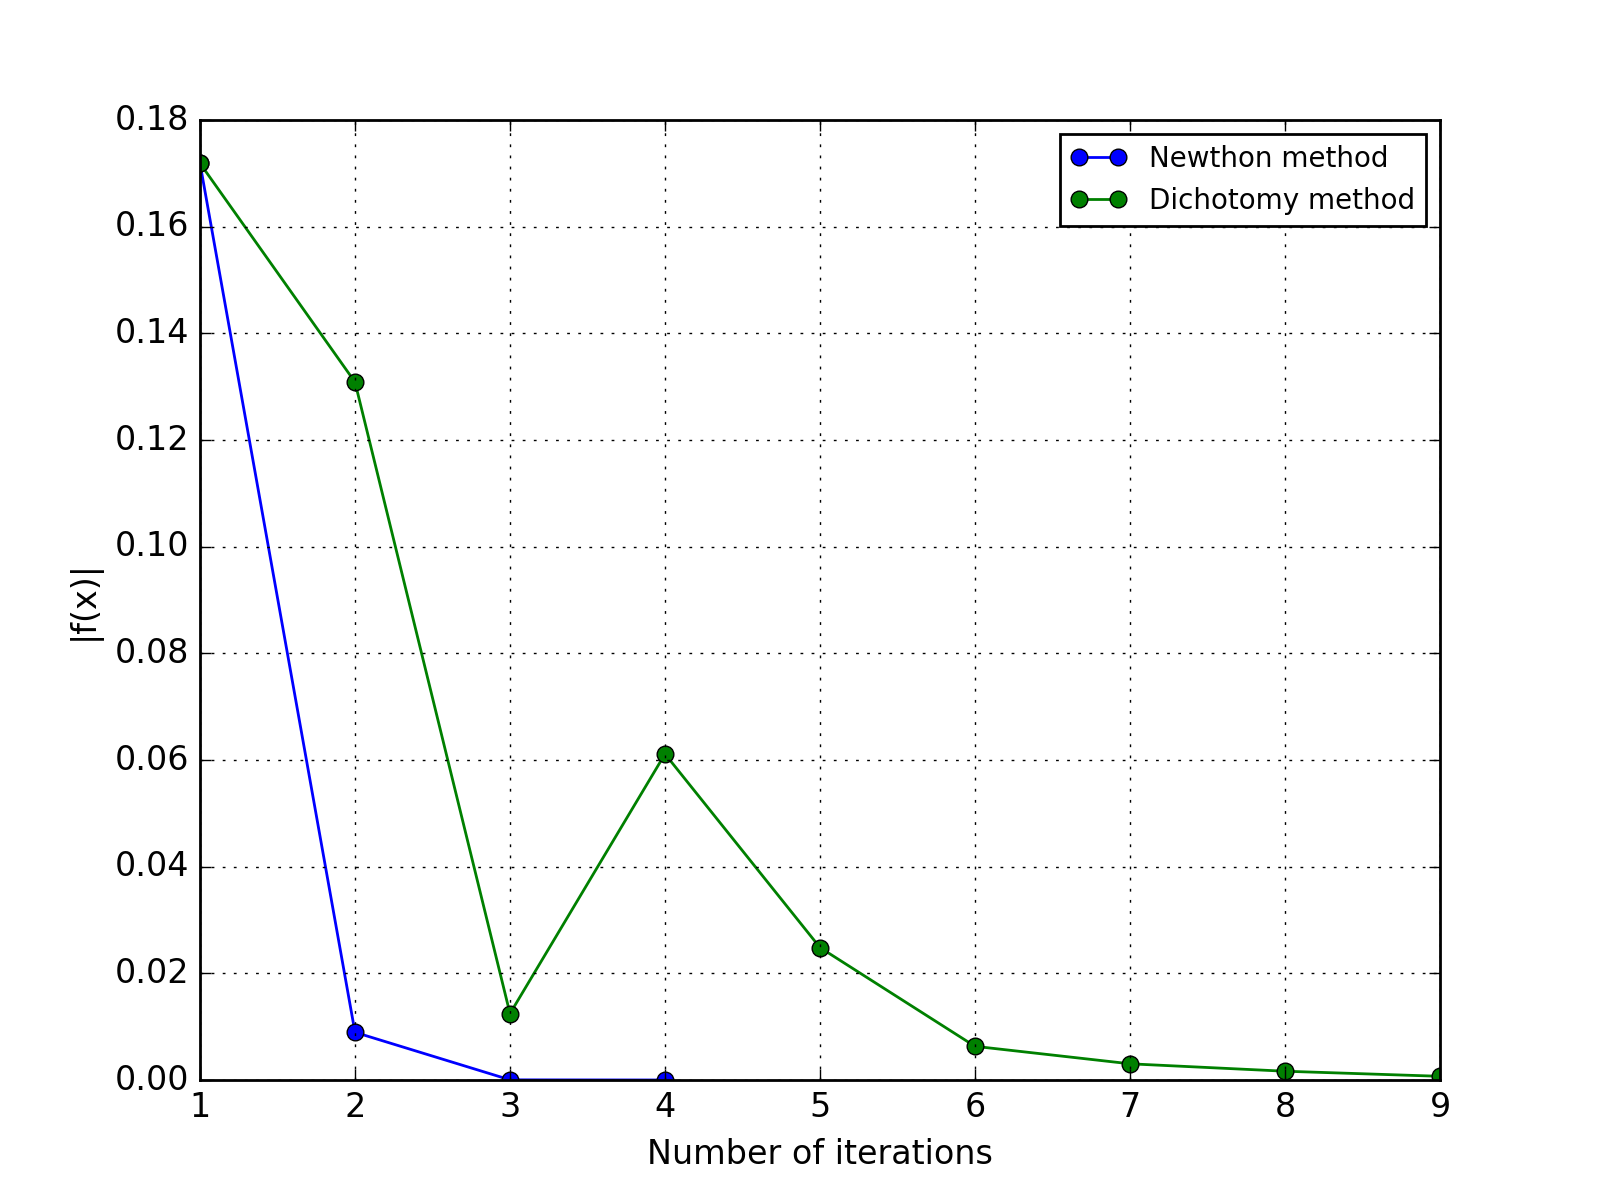
\includegraphics[width=0.75\textwidth]{../pictures/lab1_convergence.png}
  \caption{Зависимость абсолютного значения полинома от номера итерации метода}
  \label{fig:convergence}
\end{figure}

В результате запуска методов было получено приближённое значение корня
\(\widetilde{x}=0.6816\) (значение округлено). Из рис. \ref{fig:convergence} видно, что метод Нтьютона
сходится за \(4\) итерации, в то время как методу дихотомии необходимо \(9\) итераций для
достижения той же точности.

\section{Построение зависимости корня полинома от параметра}
Необходимо построить зависимость \(x^*(\alpha)\) координаты единственного корня полинома
\(f(x)=x^{N+1}+x+\alpha\) от \(\alpha\) при \(N=2,4,6\) на отрезке \([0;10]\).
Из качественного анализа положения корня следует, что при малых \(\alpha\) зависимость
схожа с линейной, а при больших --- близка к функции \(\sqrt[N+1]{\alpha}\).

Глядя на рис. \ref{fig:roots}, можно убедиться в справедливости качественных оценок.

\begin{figure}[ht]
	\center
  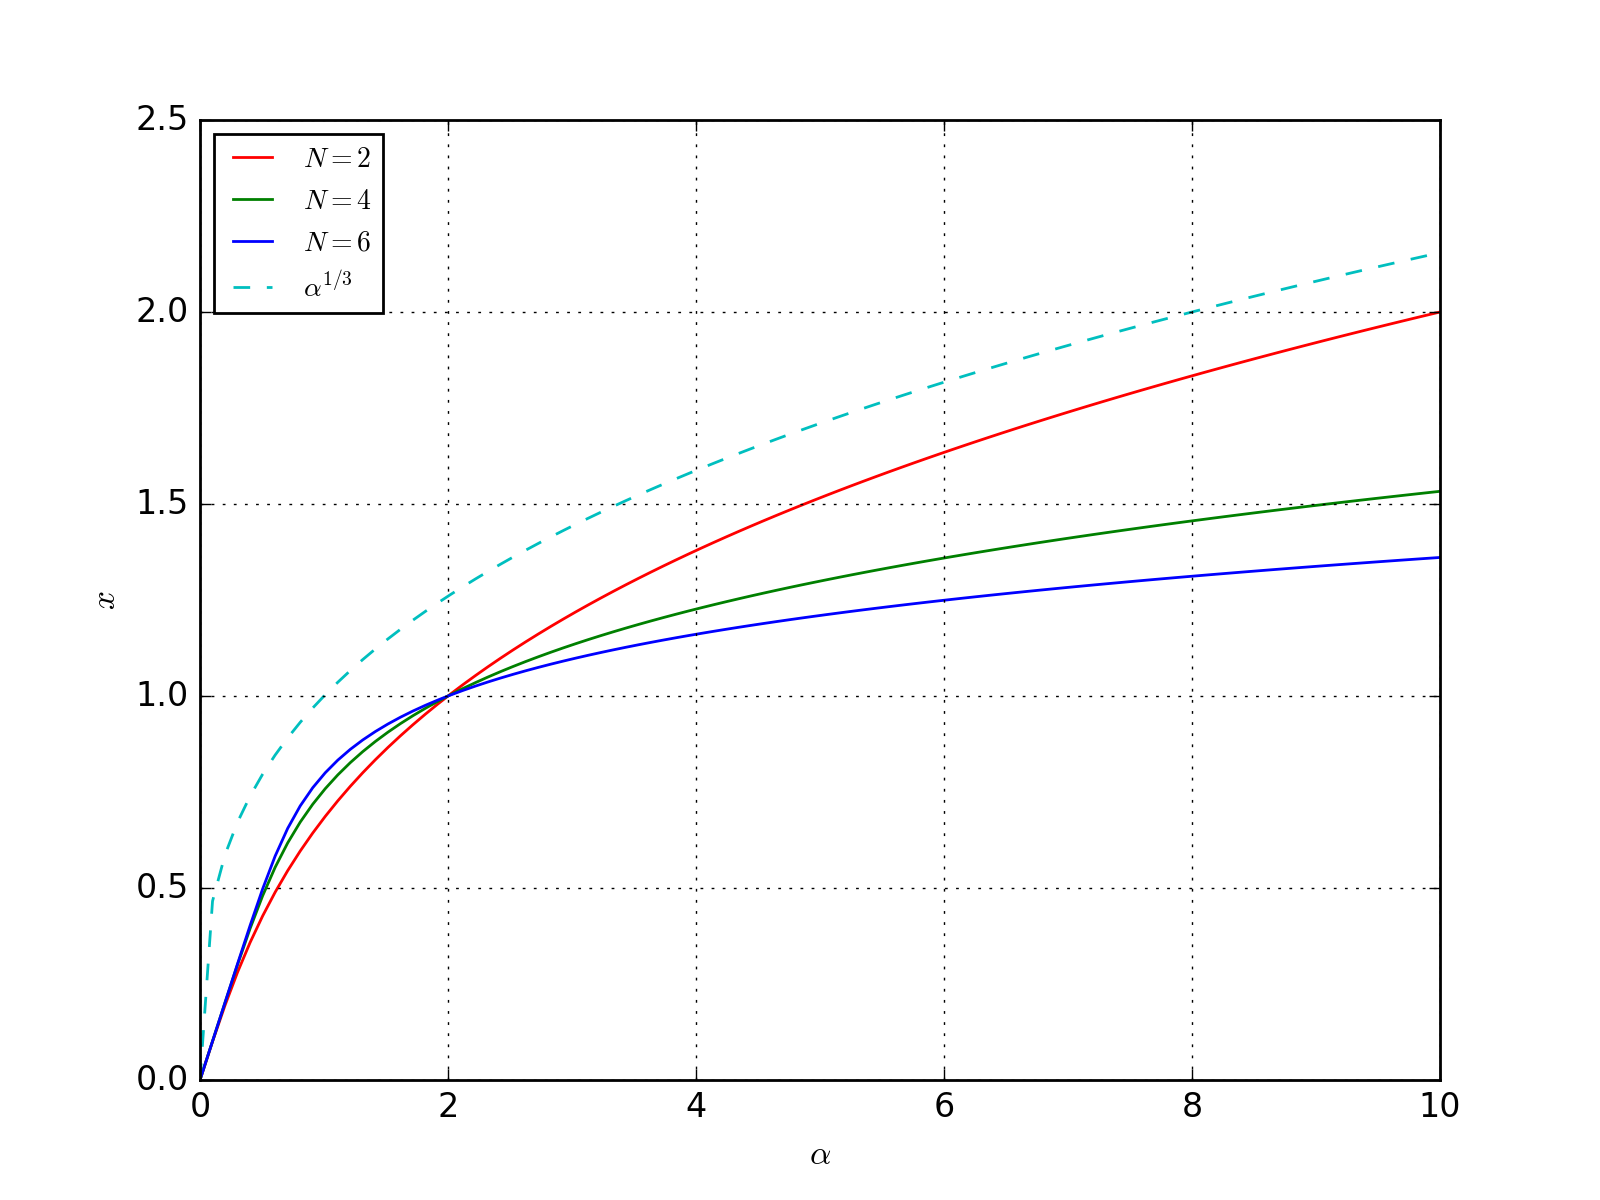
\includegraphics[width=0.75\textwidth]{../pictures/lab1_roots.png}
  \caption{Зависимость корня полинома \(f(x)\) от параметра при различных значениях степени}
  \label{fig:roots}
\end{figure}

\section{}

\lstinputlisting[language=Python, numbers=left]{../scripts/lab1.py}

\end{document}
